\documentclass{article}

\usepackage{import}
\subimport{../preamble/}{lab_preamble.tex}

\title{Capacitors, Inductors, and Complex Impedance}


\begin{document}
\maketitle

In this chapter we introduce the concept of complex resistance, or \emph{impedance}, by studying two reactive circuit elements, the \emph{capacitor} and the \emph{inductor}. We will study capacitors and inductors using differential equations and Fourier analysis and from these derive their impedance. Capacitors and inductors are used primarily in circuits involving time-dependent voltages and currents, such as AC circuits.

\section{AC Voltages and circuits}
Most electronic circuits involve time-dependent voltages and currents. An important class of time-dependent signal is the sinusoidal voltage (or current), also known as an AC signal (Alternating Current). \emph{Kirchhoff's laws and Ohm's law still apply (they always apply), but one must be careful to differentiate between time-averaged and instantaneous quantities.}

An AC voltage (or signal) is of the form:
\begin{equation}
v(t) = V_0 \cos\omega t
\end{equation}
where $\omega$ is the angular frequency, $V_0$ is the amplitude of the waveform or the \emph{peak voltage} and $t$ is the time. The angular frequency is related to the frequency $f$ by $\omega = 2 \pi f$, and the period $T$ is related to the frequency by $T = \frac{1}{f}$. Other useful voltages are also commonly defined. They include the \emph{peak-to-peak voltage} ($V_{pp}$) which is twice the amplitude $V_0$, and the RMS voltage ($V_{RMS}$) which is $V_{RMS} = V_0 / \sqrt{2}$. The average power dissipated in a resistive AC device is computed using RMS quantities:
\begin{equation}
P = I_{RMS} V_{RMS} = \frac{1}{2} I_0 V_0.
\end{equation}
This is important enough that voltmeters and ammeters in AC mode actually return the RMS values for current and voltage.

While most real world signals are not sinusoidal, AC signals are still used extensively to characterize circuits through the technique of Fourier analysis.

\subsection{Fourier Analysis}
One convenient way to characterize the rate of change of a function is to write the true function as a linear combination of a set of functions that have particularly easy characteristics to deal with analytically. In this case we can consider the trigonometric functions. It turns out that we can write any function as an integral of the form
\begin{equation}
v(t) = \int v(\omega) \cos \left( \omega t + \phi(\omega) \right) d\omega
\end{equation}
where $v(\omega)$ and $\phi(\omega)$ are functions of the frequency $\omega$. This process is called Fourier analysis, and it means that any function can be written as an integral of simple sinusoidal functions. In the case of a periodic waveform this integral becomes a sum over all the harmonics of the period (i.e. all the integer multiplicative frequencies of the period).
\begin{equation}
v(t) = \sum_n A_n \cos (n\omega t + \phi_n).
\end{equation}
An implication of this mathematical fact is that \emph{if we can figure out what happens when we put pure sinusoidal voltages into a linear circuit, then we will know everything about its operation even for arbitrary input voltages.}

\subsection{Complex Notation}
In complex notation we replace our sinusoidal functions by exponentials to make the calculus and bookkeeping easier still. Then we can include both phase and magnitude
information. We'll define 
\begin{equation}
e^{j\phi} = \cos\phi + j\sin\phi,
\end{equation}
where $j^2 = -1$.

The general procedure for using this notation is:
\begin{enumerate}
\item Change your problem into complex algebra, i.e. replace $\cos\omega t$ with $e^{j \omega t}$.
\item Solve the problem.
\item Take the real part of the solution as your answer at the end.
\end{enumerate}


\section{Capacitors}
One of the most basic rules of electronics is that circuits must be complete for currents to flow. This week, we will introduce an exception to that rule.

The capacitor is actually a small break in a circuit. Try measuring the resistance of a capacitor, you will find that it is an open circuit. However, at the inside ends of the capacitor's lead, it has little plates that act as charge reservoirs where it can store charge. For short times, you do not notice that the break is there. Negative charge initially flows in to one side and out from out the other side just as if the two leads were connected. For fast signals, the capacitor ``looks'' like a short-circuit. But after a while the capacitor's reservoirs fill, the current stops, and we notice that there really is a break in the circuit.

For slow signals, a capacitor ``looks'' like an open circuit. What is fast, and what is slow? It depends on the capacitor and the rest of the circuit. This week, you will learn how to determine fast and slow for yourselves.

Capacitors serve three major roles in electrical circuits (although all three are just variations of one basic idea):
\begin{itemize}
\item Charge integrators;
\item High or low frequency filters;
\item DC isolators.
\end{itemize}

In order to perform these functions analytically, we will need to introduce a number of new concepts and some significant mathematical formalism. In this process we will also develop a number of new concepts in analyzing electronic circuits.

\subsection{Capacitance}
A capacitor is a device for storing charge and electrical energy. It consists of two parallel conducting plates and some non-conducting material between the plates, as shown in Figure~\ref{fig:capacitor}. When voltage is applied positive charge collects on one plate and negative charge collects on the other plane. Since they are attracted to each other this is a stable state until the voltage is changed again.

A capacitor's charge capacity or capacitance ($C$) is defined as:
\begin{equation}
 Q = C V
\end{equation}
which relates the charge stored in the capacitor ($Q$) to the voltage across its leads ($V$). Capacitance is measured in Farads (F). A Farad is a very large unit and most applications use $\mu$F, nF, or pF sized devices. Many electronics components have small parasitic capacitances due to their leads and design.

The capacitor also stores energy in the electric field generated by the charges on its two plates. The potential energy stored in a capacitor with voltage $V$ on it is
\begin{equation}
 E = \frac{1}{2} C V^2
\end{equation}
We usually speak in terms of current when we analyze a circuit. By noting that the current is the rate of change of charge, we can rewrite the definition of capacitance in terms of the current as:
\begin{eqnarray}
v & = & \frac{q}{C} = \frac{1}{C} \int i dt \\
i & = & C \frac{dv}{dt} = C \dot{v}
\end{eqnarray}
This shows that we can integrate a function $i(t)$ just by monitoring the voltage as the current charges up a capacitor, or we can differentiate a function $v(t)$ by putting it across a capacitor, and monitoring the current flow when the voltage changes.

\begin{figure}
\begin{center}
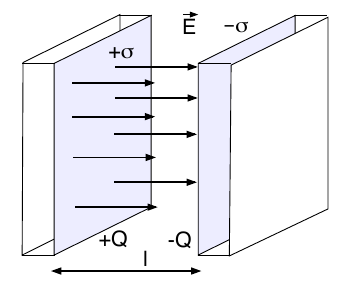
\includegraphics[width=0.4\textwidth]{pics/capacitor}
\end{center}
\caption{ A capacitor consist of two parallel plates which store equal and opposite amounts of charge.}
\label{fig:capacitor}
\end{figure}

\subsection{A Simple RC Circuit}

We will start by looking in detail at the simplest capacitive circuit, which is shown in Figure~\ref{fig:RC_circuit}. An RC circuit is made by simply putting a resistor and a capacitor together as a voltage divider. We will put the resistor in first, so we can connect the capacitor to ground.

By applying Kirchhoff's Laws to this circuit, we can see that:
\begin{itemize}
\item The same current flows through both the resistor and the capacitor, and
\item The sum of the voltage drops across the two elements equal the input voltage.
\end{itemize}
This can be put into a formula in the following equation:
\begin{equation}
v_{in} = i R + \frac{1}{C} \int i dt
\end{equation}
which can also be written as
\begin{equation}
\frac{v_{in}}{R} = i + \frac{1}{RC} \int i dt
\end{equation}
We can also put this into the form of a differential equation in the following way:
\begin{eqnarray}
\frac{dv_{in}}{dt} & = & R \frac{di}{dt} + \frac{i}{C}  \nonumber \\
C \dot{v}_{in} & = & R C \dot{i} + i
\label{eqn:RC_diffeqn}
\end{eqnarray}
These equations show that times are measured in units of $RC$, and that what you see depends on how quickly things change during one $RC$ time interval.

If the current changes quickly, then most of the voltage will show up across the resistor, while the voltage across the capacitor slowly charges up as it integrates the current. If the voltage changes slowly, then most of the voltage shows up across the capacitor as it charges. Since this usually requires a small current, the voltage across the resistor stays small.

But, what happens at intermediate times? To determine this quantitatively we will have to develop some more sophisticated mathematical techniques.

\subsection{Solutions to $RC$ Circuit}
Rather than produce the general solution, we will concentrate on two special cases that are particularly useful. The first will be for a constant voltage and the second will be a sinusoidal input.

\begin{figure}
 \begin{center}
  \begin{circuitikz}
   \draw (-2,0) node[ground]{} to[battery1,l=$v_{in}$] (-2,2) to[R,l=$R$] (0,2) to[C,l=$C$] (0,0) node[ground]{};
   \draw (0,2) to[short,-o] (1,2) node[right]{$v_{out}$};
  \end{circuitikz}
 \end{center}
 \caption{A simple RC circuit which integrates current.}
 \label{fig:RC_circuit}
\end{figure}

To study a constant supply voltage on an RC circuit, we set the left side of equation~\ref{eqn:RC_diffeqn} equal to a constant voltage. Then we have a simple homogeneous differential equation with the simple solution for the current of a decaying exponential,
\begin{equation}
 i = I_0 e^{-t/RC}
\end{equation}
which will account for any initial conditions. After a time of a few RC time periods, this solution will have decayed away to the supply voltage.

And now let us consider the other solution. In the prior section, we argued that if we can understand the $RC$ circuit's behavior for sinusoidal input we can deal with any arbitrary input. Therefore, this is the important one.

Let's look at our simple $RC$ circuit and suppose that we apply (or drive) a simple sine wave into the input:
\begin{equation}
v_{in} = V_0 \cos \omega t
\label{eqn:RC_voltage_cos}
\end{equation}
In complex notation, this means that we will set the drive voltage to
\begin{equation}
v_{in} = \Re \left(V_0 e^{j \omega t}\right)
\label{eqn:RC_voltage_exp}
\end{equation}
and we just have to remember to take the real part at the end of our calculation.

If we put this drive voltage into the differential equation \ref{eqn:RC_diffeqn}, then it becomes a relatively simple inhomogeneous differential equation:
\begin{equation}
C \frac{dv_{in}}{dt} = j \omega C V_0 e^{j \omega t} = R C \frac{di}{dt} + i.
\end{equation}
This is relatively simple because it shows up so often in physics that you might as well memorize the solution or at least the way to get the solution. Note that mathematically it looks just like a driven harmonic oscillator.

We can obtain the solution by using the standard recipe for first order linear differential equations. We start by rewriting equation as
\begin{equation}
\frac{di}{dt} + \frac{1}{R C} i = j \omega \frac{1}{R} V_0 e^{j \omega t}
\end{equation}
which we then multiply by $e^{t/RC}$ to obtain
\begin{equation}
e^{t/RC} \frac{di}{dt} + e^{t/RC} \frac{1}{R C} i = j \omega \frac{1}{R} V_0 e^{j \omega + \frac{1}{RC} t}.
\end{equation}

The left hand-side of this equality can be rewritten under the form of a total derivative (multiplication rule) so that we now have
\begin{equation}
\frac{d}{dt}\left[ i(t) e^{\left(t/RC\right)}\right] = \frac{j\omega V_0}{R} e^{\left( j\omega t + t/RC \right)}.
\end{equation}
This equation is easily integrable and can be rewritten as
\begin{equation}
i(t) e^{\left(t/RC\right)} = \frac{j\omega V_0}{R} \int e^{\left(j\omega t + t/RC\right)} dt.
\end{equation}
The integral is straightforward and yields the following expression:
\begin{equation}
i(t) = \frac{j\omega V_0}{R} \frac{1}{\frac{1}{RC} + j\omega} e^{\left(j\omega t\right)} + \hbox{constant} \cdot e^{\left( -t/RC \right)}.
\end{equation}
The first term represents the ``steady state'' oscillatory behavior of the driven circuit, while the second term describes the transient behavior of the current after switching on the driving voltage. Since we are only interested in the long-term behavior of the circuit, we neglect the second term and concentrate on the first. After a little bit of algebra, we can rewrite the steady-state current as
\begin{equation}
i(t) = \frac{j\omega V_0}{R} \frac{1}{\frac{1}{RC} + j\omega} e^{\left(j\omega t\right)} = \frac{\omega V_0 C}{\sqrt{1 + (\omega RC)^2}} \frac{\omega RC + j}{\sqrt{1 + (\omega RC)^2}} e^{\left(j\omega t\right)}.
\end{equation}
The second fraction can be interpreted as a phase term with $\tan\phi = \frac{1}{\omega RC}$, so that the expression for the current becomes
\begin{equation}
i(t) = I_0 e^{\left(j\omega t + \phi\right)}
\label{eqn:current_in_RC_circuit}
\end{equation}
with
\begin{equation}
I_0 = \frac{\omega V_0 C}{\sqrt{1 + \left(\omega RC\right)^2}} = \frac{V_0}{R} \cos\phi.
\end{equation}
The real solution of this simple RC circuit can be obtained by taking the real part of equation~\ref{eqn:current_in_RC_circuit}, and is left as an exercise to the reader.

The solution of the simple RC circuit appears to be rather complicated and involved, however it simplifies considerably when we plug equation~\ref{eqn:current_in_RC_circuit} back in to the original integral equation from Kirchhoff's loop law (equation~\ref{eqn:RC_diffeqn}). After integrating the exponential and a little bit of algebra, we obtain
\begin{equation}
v_{in}(t;\omega) = i(t) R + i(t) \frac{1}{j\omega C}
\end{equation}
This remarkably simple expression looks a lot like the standard Kirchhoff's loop law for resistors, except that the capacitor term behaves with a frequency dependent ``imaginary'' resistance.

\subsection{RC Impedance}
We will obtain the same solution as the one we obtained for the original voltage divider, as long as we assign an imaginary, frequency dependent, resistance to the capacitor. The ``imaginary'' part just means that it will produce a $\pi/2$ phase shift between the voltage and the current for a sinusoidal input. We will call this impedance
\begin{equation}
Z_C = \frac{1}{j \omega C}
\end{equation}

Now, the solution for an RC divider becomes somewhat simplified. We can compute the total current flowing through the circuit as
\begin{equation}
i = \frac{v_{in}}{Z_{tot}} = \frac{v_{in}}{R + Z_C} = \frac{V_0 e^{j\omega t}}{R + \frac{1}{j\omega C}} = \frac{j\omega C V_0 e^{j\omega t}}{1 + j\omega RC} = \frac{V_0}{R} \frac{j\omega RC e^{j\omega t}}{1 + j\omega RC} = \frac{V_0}{R} e^{j\omega t}  \cos\phi.
\end{equation}
The voltage across an element is just this current times the element's impedance. For the
voltage drop across the resistor it is largely the same as before:
\begin{equation}
v_R = i R = V_0 \cos\phi e^{j\left(\omega t + \phi\right)}
\end{equation}
For the capacitor, we get the following voltage drop:
\begin{eqnarray}
v_C = i Z_C = \frac{I}{j\omega C} & = & \frac{V_0 \cos\phi e^{j\left(\omega t + \phi\right)}}{j\omega RC} = -j V_0 \sin\phi e^{j\left(\omega t + \phi\right)} \\
& = & V_0 \frac{\cos\phi}{\omega RC} e^{j\left(\omega t + \phi + \pi/2\right)} = V_0 \sin\phi e^{j\left(\omega t + \phi + \pi/2\right)}.
\end{eqnarray}
If everything is correctly calculated then the sum of the voltage drops across the two elements should be equal to the input voltage. Let's try it:
\begin{equation}
v_R + v_C = V_0 \left( \cos\phi - j\sin\phi \right) e^{j\left(\omega t + \phi\right)} = V_0 e^{-j\phi} e^{j\left(\omega t + \phi\right)} = V_0 e^{j\omega t}.
\end{equation}
Remember, you get the actual waveforms by taking the real parts of these complex solutions. Therefore
\begin{eqnarray}
v_R & = & V_0 \cos\phi \cos(\omega t + \phi) \\
v_C & = & V_0 \sin\phi \cos(\omega t + \phi - \pi/2) = - V_0 \sin\phi \sin(\omega t + \phi)
\end{eqnarray}
This looks complicated, but the limits of high frequency and low frequency are easy to remember. At high frequencies ($\phi \to 0$), the capacitor is like a short, and all the voltage shows up across the resistor. At low frequencies ($\phi \to \pi/2$), the capacitor is like an open circuit, and all the voltage shows up across the capacitor.
If you consider the leading terms for the elements with the small voltages, you find that
\begin{eqnarray}
v_C & = & V_0 \frac{1 - j\omega RC}{1 + (\omega RC)^2} \to -\frac{j}{\omega} \frac{V_0}{RC} \quad \hbox{as}~\omega \to \infty, \\
v_R & = & V_0 \frac{\omega RC \left(1 + j\omega RC\right)}{1 + (\omega RC)^2} \to j\omega RC V_0 \quad \hbox{as}~\omega \to 0.
\end{eqnarray}
Thus, at high frequency, the voltage across the capacitor is the integral of the input voltage, while at low frequency the voltage across the resistor is the derivative of the input voltage. 

This says that as long as all the important frequencies are high, the capacitor will integrate the input voltage. If all the important frequencies are small, the resistor will differentiate the voltage. If there are intermediate frequencies, or a mixture of some high and some low frequencies, the result will not be so simple but it can be determined from the voltage divider algebra using complex notation.

We finish by noting that the voltage on the capacitor is always $-\pi/2$ out of phase with the voltage on the resistor.

\section{Inductors}

\begin{figure}
\begin{center}
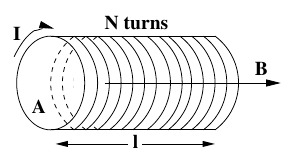
\includegraphics[width=0.5\textwidth]{pics/inductor}
\end{center}
\caption{An inductor consists of a coiled wire, also called a solenoid. The arrow $B$ represent the magnetic field generated by the current $I$ in the inductor.}
\label{fig:inductor}
\end{figure}

An inductors is a coil of wire, or solenoid, which can be used to store energy in the magnetic field that it generates (see Figure~\ref{fig:inductor}). It is mathematically similar to a capacitor, but has exactly the opposite behavior: it behaves as a short circuit for low frequencies and as an open circuit for high frequencies (i.e. it passes low frequency signals and blocks high frequency signals).

The energy stored in the field of an inductor with inductance $L$ is given by the following formula:
\begin{equation}
 E = \frac{1}{2} L I^2
\end{equation}
The SI unit of inductance is the Henry (H). Commercially available inductors have inductances that range from nH to mH. Small millimeter-size and centimeter size solenoids typically have inductances in the range of $\mu$H, while magnetic field coils can have a inductances in the mH range, and can sometimes have inductances of up to several H. Most electronics components have small parasitic inductances due to their leads and design (for example, wire-wound power resistors).

In an electric circuit, a voltage, or electromotive potential, is generated across the terminals of the inductor when the current changes due to Faraday's law. The voltage drop is given by the following simple expression:
\begin{equation}
v = L \frac{di}{dt}
\end{equation} 
From this equation, we see that the inductor operates exactly opposite to a capacitor: an inductor differentiates the current and integrates the voltage.

\subsection{The \boldmath$LR$ circuit}

\begin{figure}
 \begin{center}
  \begin{circuitikz}
   \draw (-2,0) node[ground]{} to[battery1,l=$v_{in}$] (-2,2) to[R,l=$R$] (0,2) to[L,l=$L$] (0,0) node[ground]{};
   \draw (0,2) to[short,-o] (1,2) node[right]{$v_{out}$};
  \end{circuitikz}
 \end{center}
 \caption{A simple LR circuit.}
 \label{fig:LR_circuit}
\end{figure}

We can analyze the $LR$ circuit in much the same way that we derived the operation of the $RC$ circuit. We start by applying Kirchhoff's loop law to the $LR$ circuit in Figure~\ref{fig:LR_circuit}, and we find that
\begin{equation}
v_{in} = i R + L \frac{di}{dt}.
\end{equation}
If we apply a constant voltage $V_0$ the solution can be calculated using the techniques developed for the $RC$ circuit and we calculate that
\begin{equation}
i(t) = I_0 \left(1 - e^{\left(-\frac{R}{L}t\right)}\right).
\end{equation}
The circuit approaches the steady state current $I_0 = V_0 / R$ with a time constant of $L / R$.

\subsection{$LR$ impedance}
Instead of solving the differential equation for the $LR$ circuit with a sinusoidal applied input voltage such as that given by equations~\ref{eqn:RC_voltage_cos} and~\ref{eqn:RC_voltage_exp}, as we did with the $RC$ circuit, we will just assume that the current has the form
\begin{equation}
i(t) = I_0 e^{(j\omega t + \phi)}.
\end{equation}
We plug this ansatz solution back into the differential equation and find that
\begin{equation}
v_{in} = i(t) R + j \omega L i,
\end{equation}
from which we deduce that the inductor behaves as a resistor with frequency dependent ``imaginary'' resistance. The impedance of an inductor is therefore
\begin{equation}
Z_L = j \omega L.
\end{equation}
Just as with the RC circuit, we can apply Ohm's law to the circuit to calculate the total current. Since R and L are in series, we obtain
\begin{equation}
i(t) = \frac{v_{in}}{Z_{tot}} = \frac{V_0 e^{j\omega t}}{R + Z_L} = \frac{V_0}{R} \frac{1 - j\omega L/R}{1 + \left(\omega \frac{L}{R}\right)^2} e^{j\omega t} = \frac{V_0}{R} \cos\phi e^{j(\omega t - \phi)}
\end{equation}
where the phase is given by $\tan\phi = \omega\frac{L}{R}$. We calculate the voltage drop across the resistor using the expression for the current and find that
\begin{equation}
v_R = i(t) R = V_0 \cos\phi e^{j(\omega t - \phi)}.
\end{equation}
The voltage drop across the inductor is calculated the same way, and we find
\begin{equation}
v_L = j\omega L i(t) = j\omega L \frac{V_0}{R} \cos\phi e^{j(\omega t - \phi)} = j V_0 \sin\phi e^{j(\omega t - \phi)} = V_0 \cos\phi e^{j(\omega t - \phi + \pi/2)}.
\end{equation}

If everything is correctly calculated then the sum of the voltage drops across the two elements should be equal to the input voltage. Let's try it:
\begin{equation}
v_R + v_L = V_0 \left( \cos\phi + j\sin\phi \right) e^{j(\omega t - \phi)} = V_0 e^{j\phi} e^{j(\omega t - \phi)} = V_0 e^{j\omega t}.
\end{equation}
You get the actual waveforms by taking the real parts of these complex solutions.
Therefore
\begin{eqnarray}
v_R & = & V_0 \cos\phi \cos(\omega t - \phi), \\
v_L & = & V_0 \sin\phi \cos(\omega t - \phi + \pi/2) = V_0 \sin\phi \sin(\omega t - \phi). 
\end{eqnarray}
This looks complicated, but the limits of high frequency and low frequency are easy to remember. At high frequencies ($\phi \to \pi/2$), the inductor is like an open circuit, and all the voltage shows up across the inductor. At low frequencies ($\phi \to 0$), the inductor is like a short circuit or just a plain wire, and all the voltage shows up across the resistor.

It should also be pointed out that the voltage on the inductor is always $+\pi/2$ out of phase with the voltage on the resistor.

\section{Transformers}
Transformers are an ingenious combination of two inductors. They are used to transfer power between two circuits by magnetic coupling. The transformer changes an input voltage, without affecting the signal shape, similar to the voltage divider of last week. However it has several important differences:
\begin{enumerate}
\item It can increase as well as decrease a signal's amplitude (i.e. AC voltage).
\item It requires a time-varying (AC) input to work.
\item It is much harder to fabricate.
\item It usually does not work well for very fast
signals (since inductors block high frequencies).
\end{enumerate}

Transformers are commonly used as a major component in a DC power supplies since they can convert a 120\,V AC wall voltage into a smaller voltage that is closer to the desired DC voltage (e.g. 5\,V or $\pm 15$\,V). The schematic symbol for a transformer is shown in Figure~\ref{fig:transformer}.

Transformers are passive devices that simultaneously change the voltage and current of a circuit. They have (at least) four terminals: two inputs (called the primary) and two outputs (called the secondary). There is no real difference between the input and output for a transformer, you could simply flip it around and use the secondary as the input and the primary as the output. However, for the sake of clarity, we will always assume that you use the primary for input and the secondary for output.

\begin{figure}
 \begin{center}
  \begin{circuitikz}
   \draw (0,0) node[transformer](T){};
  \end{circuitikz}
  \caption{The schematic symbol for a transformer.}
  \label{fig:transformer}
 \end{center}
\end{figure}

The coupling between the input and output is done magnetically. This allows transformers to have a number of interesting benefits including:
\begin{enumerate}[resume]
\item There is no DC connection between input and output, so transformers are often used to isolate one circuit from another.
\item Transformers only work for time varying signals, when the inductive coupling between the coils is greater than the resistive losses.
\end{enumerate}
Since they have no external power the output power cannot be greater than the input power
\begin{equation}
P = v_P i_P \ge v_S i_S.
\end{equation}
Usually, we will assume equality but there are small resistances (and hence resistive losses) in the coils and a poorly or cheaply designed transformer many not have the input and output sufficiently strongly coupled to each other. Depending on the device and the signal the output power may well be less than the input power.

Transformers are most commonly used to change line voltage (120\,V RMS at 60\,Hz) into a more convenient voltage. High power transmission lines use transformers to increase the voltage and decrease the current. This reduces $i^2 R$ power losses in the transmission wires. For our circuits we will use a transformer that reduces the voltage and increases the current.

Transformers are characterized by the ratio of the number of turns on the input and output windings. The magnetic coupling in an ideal transformer will insure that the number of turns times the current flowing is the same for the input and output:
\begin{equation}
N_P i_P = N_S i_S \Rightarrow \frac{i_S}{i_P} = \frac{N_P}{N_S}
\end{equation}
Since the voltage must change in the opposite manner to keep the input and output power, the ratio of the voltages is the same as the ratio of the turns:
\begin{equation}
\frac{v_S}{v_P} = \frac{N_S}{N_P}.
\end{equation}
Transformers are usually called step-up or step-down according to whether the output voltage increases or decreases.

A transformer also transforms the impedance of a circuit, since it changes the ratio of $v/i$. Using our rules above, the ratio of output impedance to input impedance is the square of the ratio of turns:
\begin{equation}
\frac{Z_S}{Z_P} = \frac{v_S}{i_S} \frac{i_P}{v_P} = \left(\frac{N_S}{N_P}\right)^2.
\end{equation}
So, if you use a transformer as a step-up transformer, it increases the voltage and the impedance at its output relative to its input. If you use a transformer as a step-down transformer, it decreases the voltage and the impedance at its output.

A similar relationship is valid when a voltage source $v_{in}$ with internal impedance $Z$ is connected to the primary terminals of a transformer, and the whole assembly is treated as a black box with new internal impedance $Z'$, as shown in Figure~\ref{fig:transformer_effective_impedance}.

\begin{figure}
 \begin{center}
  \begin{subfigure}[b]{0.48\textwidth}
   \begin{center}
    \begin{circuitikz}
     \draw (0,0) node[transformer](T){};
     \draw (T.A2) to[short] ($(T.A2)-(2,0)$) to[sinusoidal voltage source,l=$v_{in}$] ($(T.A1)-(2,0)$) to[generic,l=$Z$] (T.A1);
     \draw (T.B1) to[short,-o] ($(T.B1)+(0.1,0)$);
     \draw (T.B2) to[short,-o] ($(T.B2)+(0.1,0)$);
    \end{circuitikz}
   \end{center}
   \caption{Voltage source with internal impedance $Z$ connected to a transformer.}
  \end{subfigure}\quad%
  \begin{subfigure}[b]{0.48\textwidth}
   \begin{center}
    \begin{circuitikz}
     \draw (0,0) to[sinusoidal voltage source,l=$v'_{in}$] (0,2) to[generic,l=$Z'$] (2,2) to[short,-o] (2.1,2);
     \draw (0,0) to[short,-o] (2.1,0);
    \end{circuitikz}
   \end{center}
   \caption{Equivalent voltage source with effective internal impedance $Z'$.}
  \end{subfigure}
  \caption{Effective internal impedance of a voltage source connected to the primary coil of a transformer.}
  \label{fig:transformer_effective_impedance}
 \end{center}
\end{figure}


\pagebreak

\section{Lab 3: Design Exercises}

\begin{enumerate}
\item Using Kirchhoff's laws, derive a formula for the total capacitance of two capacitors in parallel and a formula for the total capacitance of two capacitors in series. (Hint: pretend that you are working with an AC signal of frequency $\omega$).
\item Using Kirchhoff's laws, derive a formula for the total inductance of two inductors in parallel and a formula for the total inductance of two inductors in series. (Hint: pretend that you are working with an AC signal of frequency $\omega$).
\item Calculate $v_{out}$ as a function of $v_{in}$ in the $RLC$ circuit in Figure~\ref{fig:RLC_filter1}, using the formulas for $Z_R$, $Z_C$, and $Z_L$. Assume that $v_{in}$ is a perfect AC voltage signal with a frequency of $\omega$.  (Do not use Maple / Mathematica / MATLAB / MathCad for these calculations and show all steps.)

Plot the magnitude and phase\footnotemark{} of $v_{out}/v_{in}$ as a function of $\omega$ for $R = 1$\,k\Ohm, $C = 1$\,$\mu$F, and $L = 10$\,$\mu$H. What happens to the magnitude and the phase of $v_{out}$ at $\omega = \frac{1}{\sqrt{LC}}$?  (Maple / Mathematica / MATLAB / MathCad are permitted for the
plots.)

\footnotetext{Use a logarithmic scale for the frequency $\omega$, a logarithmic scale for the magnitude, and a linear scale for the phase.}

\item Calculate $v_{out}$ as a function of $v_{in}$ in the $RLC$ circuit in Figure~\ref{fig:RLC_filter2}, using the formulas for $Z_R$, $Z_C$, and $Z_L$. Assume that $v_{in}$ is a perfect AC voltage signal with a frequency of $\omega$.  (Do not use Maple / Mathematica / MATLAB / MathCad for these calculations and show all steps.)

Plot the magnitude and phase of $v_{out}/v_{in}$ as a function of $\omega$ for $R = 1$\,k\Ohm, $C = 1$\,$\mu$F, and $L = 10$\,$\mu$H. What happens to the magnitude and the phase of $v_{out}$ at $\omega = \frac{1}{\sqrt{LC}}$?  (Maple / Mathematica / MATLAB / MathCad are permitted for the plots.)

\item Determine the effective internal impedance $Z'$ of the voltage measured at the secondary terminals of a an ideadl transformer when a voltage source $v_{in}$ with actual internal impedance $Z$ is connected to the primary terminals, as depicted in Figure~\ref{fig:transformer_effective_impedance}.
\label{ex:transformer}
\end{enumerate}

\begin{figure}
 \begin{center}
  \begin{subfigure}{0.5\textwidth}
   \begin{center}
   \begin{circuitikz}
    \draw (-2,2) node[left]{$v_{in}$} to[R,l=$R$,o-] (0,2) to[C,l=$C$] (0,0) to[L,l=$L$] (0,-2) node[ground]{};
    \draw (0,2) to[short,-o] (1,2) node[right]{$v_{out}$};
   \end{circuitikz}
   \end{center}
   \caption{An RLC filter circuits.}
   \label{fig:RLC_filter1}
  \end{subfigure}%
  \begin{subfigure}{0.5\textwidth}
   \begin{center}
   \begin{circuitikz}
    \draw (-2,2) node[left]{$v_{in}$} to[R,l=$R$,o-] (0,2) to[short] (0,1) to[short] (-1,1) to[C,l=$C$] (-1,-1) to[short] (0,-1) to[short] (0,-2) node[ground]{}; 
    \draw (0,1) to[short] (+1,1) to[L,l=$L$] (+1,-1) to[short] (0,-1);
    \draw (0,2) to[short,-o] (1,2) node[right]{$v_{out}$};
   \end{circuitikz}
   \end{center}
   \caption{Another RLC filter circuits.}
   \label{fig:RLC_filter2}
  \end{subfigure}
 \end{center}
\caption{Two RLC filter circuits.}
\label{fig:RLC_filter}
\end{figure}

\section{Lab 3: AC signals, Complex Impedance, and Phase}

\subsection{Introduction to transformers}
In this section, we use a transformer to change the impedance of an AC signal.
\begin{enumerate}
\item Measure the output impedance of a signal generator with a 0.5\,V amplitude sinusoid output of 1\,kHz. Remember you are using AC signals. Pay no attention to the DC voltage and current offset. In fact, try to null them with the signal generator offset knob. What does an AC current reading from a DVM mean in terms of the waveform? Check this with the oscilloscope. If measurements do not match call instructor for discussion before you proceed any further.
\item Connect a transformer to the signal generator. Use terminals marked ``1'' and ``2'' as the primary, and the terminals marked ``3'' and ``4'' as the secondary (i.e. output). Measure the $v_{out}/v_{in}$ ratio. Based on this, estimate the ratio of turns. Using theoretical formula estimate the expected output impedance of the signal generator and transformer combo (transformer must be hooked such as to decrease the output voltage and increase the output current).
\item Recall that for output impedance measurement, it is good idea to have a total load resistance comparable with internal resistance of the device under test (``DUT''). Measure the resistance of the multimeter when it is set to measure current (do it for mA and $\mu$A ranges). Is it good idea to use it for the output impedance estimation of the signal generator and transformer combo? How do you measure current with an oscilloscope? Remember that the oscilloscope has a reference terminal internally wired to the ground.
\item Measure the output impedance of the signal generator plus transformer circuit. Does the measured value agree with what you expect theoretically?  How would you modify your determination in design exercise~\ref{ex:transformer} to account for realistic transformers?
\end{enumerate}

\subsection{Capacitors in series and parallel}
In this section, we take a first look at the classic $RC$ circuit and the concept of phase.
\begin{enumerate}[resume]
\item Get two capacitors and measure their individual capacitances. Measure the total capacitance with a capacitance meter when they are in series, and when they are in parallel. Is it in agreement with your expectation?
\end{enumerate}

\subsection{The \boldmath$RC$ circuit (Bonus)}

\begin{figure}
 \begin{center}
  \begin{circuitikz}
   \draw (-2,2) node[left]{$v_{in}$} to[R,l=$R$,o-] (0,2) to[C,l=$C$] (0,0) node[ground]{};
   \draw (0,2) to[short,-o] (1,2) node[right]{$v_{out}$};
  \end{circuitikz}
  \caption{An RC filter circuit.}
  \label{fig:rc_filter}
 \end{center}
\end{figure}

\begin{enumerate}[resume]
\item Construct the $RC$ circuit in Figure~\ref{fig:rc_filter}, with component ranges $R = 1-10$\,k\Ohm and $C = 0.001-0.01$\,$\mu$F. Set the function generator at approximately $\omega = 0.1/RC$ with a square wave and describe what you see. Measure the time constant of the exponential and use it to determine the capacitance of $C$ ($R$ should be determined with a multimeter).
\item (Same set-up) Set the function generator to sinusoidal output at $\omega = 1/RC$ (notice that $\omega \ne f$) and measure the magnitude of $v_{in}$ and $v_{out}$. Do you get what you expect ? Measure the phase of $v_{out}$ with respect to $v_{in}$ and make a Lissajous plot of $v_{out}$ and $v_{in}$ (ask your instructor how to do it).
\end{enumerate}

\end{document}
